\section{Objective}
Rewrite and compare the current sources, simple mirror, cascode, high-swing cascode, Wilson, modified Wilson, regulated and complete regulated mirrors in Chapter 1, ``Current Sinks and Sources,'' of \textit{AIC Lab.pdf} (physical PDF pages 2--21). This delivery previews AIC Lab 1 only. Existing code supplies geometry and provenance references; the handout's circuits, questions and measurements define the coverage checklist.

The model library, supplied separately by the user, is used at 1.0 V. The handout's 0.35 $\mu$m, 3.3 V model, threshold and numerical plots are not acceptance targets for the supplied model. The 1 V supply is a teaching design condition, not a certification of the encrypted model's voltage rating.

\section{Specification Mapping}
All page numbers are physical PDF pages. ``Simulated'' means actual HSPICE data exist; it does not imply every operating point meets its design conditions. The 5\% current-error limit is an explicit comparison criterion adopted here, not a guaranteed handout specification.
\begin{longtable}{p{0.12\linewidth}p{0.38\linewidth}p{0.17\linewidth}p{0.22\linewidth}}
\toprule
Page/item & Requirement & Implementation & Status \\
\midrule\endhead
2--4 / 1.1 & N/P I--V, compliance and output resistance versus $L$ & Deck 01 & Four lengths and gate sweeps simulated \\
5--7 / 1.2 & 50 $\mu$A; ratios 2/4/8/16; outputs 1/0.6/0.3/0.1 V & Deck 02 & Original geometry retained; low-voltage errors measured \\
7 / 1.4 & Unit-size matching and M0--M4 layout & Section 6 & Analytical answer; no completed layout claimed \\
8--10 / 2.1 & Cascode current, headroom and $R_o$ & Deck 03 & Original case exceeds rail; resized case separate \\
10--12 / 2.2, 2.4 & High swing, M4 sizing and current error & Deck 04, section 6 & Bias-length and current variants simulated \\
13--16 / 3.1--3.3 & Wilson and modified Wilson current/resistance & Deck 05 & Compared at the same operating point \\
17 / 3.4 & Swap diode-connected branches; compare $R_o$ order & Deck 05, section 6 & Failing swapped case retained \\
18--19 / 4.1 & Regulated cascode and extra bias branch & Deck 06 & Current, bias and regions checked \\
20 / 4.2 & Complete regulated cascode & Deck 06 & Added circuit; case 4 meets declared point checks \\
21 / 4.4-Q1 & Complete comparison table & Section 5, CSV & Current error, $V_{min}$, $R_o$, power and rail margin \\
21 / 4.4-Q2 & Requested $g_m^3/g_d^5$ and drawbacks & Deck 07, section 6 & Printed units inconsistent; literal target unresolved \\
\bottomrule
\end{longtable}

\section{Circuits and Design Derivation}
\subsection{Basic Relationships and Process Differences}
Identical unit geometry and bias give the ideal current-mirror relationship
\[
\frac{I_o}{I_{ref}}\simeq\frac{(W/L)_o}{(W/L)_{ref}}=M,
\qquad r_o=\left(\frac{\partial I_D}{\partial V_{DS}}\right)^{-1}=\frac{1}{g_{ds}}.
\]
Long-channel, strong-inversion approximations give $V_{DS,min}\simeq V_{OV}$ and $r_o\simeq1/(\lambda I_D)$. For PMOS, use positive magnitudes of $V_{SD}$ and $V_{SG}$. Local negative feedback raises cascode resistance to approximately $R_o\simeq g_mr_o^2$; a regulated structure adds gain, giving an order of $g_m^2r_o^3$. These equations explain trends and do not replace the supplied model's operating points and derivatives.

The handout uses $\mu_n C_{ox}=166\,\mu\mathrm{A}/\mathrm{V}^2$, $V_T=0.55$ V, $W/L=3/1.4$ and $I_{ref}=50\,\mu$A to obtain $V_{GS}\simeq1.08$ V and $V_{OV}\simeq0.53$ V. With $\lambda=0.0209/\mathrm{V}$, its 100/200 $\mu$A branches give about 478/239 k$\Omega$. These are the original hand calculations. The reference measured with the supplied model is $V_{GS}=0.6591$ V; the old parameters and operating-region conclusions cannot simply be reused.

\subsection{Explicit Geometry and Case Definitions}
Case 0 of decks 02--06 retains $W_{unit}=3\,\mu$m, $L=1.4\,\mu$m and $I_{ref}=50\,\mu$A. Cases 1 and 2 change only the current to 10 and 1 $\mu$A. Case 3 retains 50 $\mu$A and $L=1.4\,\mu$m while widening each unit to 30 $\mu$m, reducing current density and the $V_{GS}$ required by stacked devices. This is a separate design adaptation for the supplied model, not a reproduction of the original geometry.

Deck 04 adds cases 4/5 at 1 $\mu$A and $W_{unit}=3\,\mu$m with M4 lengths of 3.5/14 $\mu$m (baseline 7 $\mu$m). Deck 06 adds case 4 with $W_{unit}=30\,\mu$m, MC2 width 120 $\mu$m and MC5/MC6 widths 300 $\mu$m; other dimensions remain as in case 3. This improves the amplifier-load headroom. The added complete-regulated PMOS dimensions are design choices here, not numerical values supplied by the handout.

\section{Simulation Setup}
Each of the seven standalone \texttt{.sp} decks directly includes the specified model and can be opened in the simulator without another subcircuit file. Actual runs used PrimeSim HSPICE S-2021.09 win64 at 27 $^\circ$C. All 30 base/alter cases completed without an error or failed measurement. Deck 01 covers four lengths, each with 11 gate voltages and 101 drain voltages.

DC output sweeps cover 0--1 V in 1 mV steps; all primary comparisons use $V_o=0.8$ V. A 1 V AC test gives $R_o=1/|I_{ac}|$ at 1 Hz. In the simple mirror, only VTEST has AC=1; the other fixed output sources have AC=0. This measures a single output-port impedance. A DC central difference at 0.799/0.801 V independently checks the result. The primary comparison cases agree within 0.56\%, with near-zero 1 Hz phase, supporting the low-frequency resistance approximation. The fixed M1--M4 table reports intrinsic device $1/g_{ds}$, a different definition from the complete output-port measurement.

Define
\[
\epsilon_I=100\left(\frac{I_o}{2I_{ref}}-1\right)\%,\qquad
P_b=V_{DD}I_{bias,supply},\qquad P_o=V_oI_o.
\]
$V_{min,5\%}$ is the lowest 1 mV grid point from which every subsequent point through 1 V satisfies $|\epsilon_I|\le5\%$ and all listed bias nodes stay within 0--1 V. This operational definition is not the theoretical saturation boundary; device regions are not certified at every sweep point. Check=Y additionally requires $|V_{DS}|\ge|V_{DSAT}|$ for every relevant MOS at 0.8 V. HSPICE Subth labels are retained and are not treated as strong inversion.

$P_b$ includes only bias-supply branches; the external ideal output-voltage source separately supplies $P_o$. Neither term includes the design cost of a physical reference-current generator. Being inside the rails is only a necessary condition: an ideal IREF can deliver its specified current with very little headroom, which does not prove a physical reference source is feasible.

HSPICE also reports suppressed warnings associated with encrypted blocks. A diagnostic run with \texttt{WARNLIMIT=100} reveals no further detail. Its measurements agree with the original run, but this does not establish that the warnings are harmless; a warning-free simulation is not claimed.

\section{Results and Specification Checks}
\subsection{Channel Length and the Original Four-Branch Example}
For $W=5\,\mu$m, $V_{GS}=V_{SG}=0.6$ V and $V_{DS}=V_{SD}=0.8$ V:

\begin{center}\small
\begin{tabular}{lrrrr}
\toprule
$L$ ($\mu$m) & $I_n$ ($\mu$A) & $|I_p|$ ($\mu$A) & $r_n$ (M$\Omega$) & $r_p$ (M$\Omega$) \\
\midrule
0.35 & 230.165 & 42.540 & 0.095 & 0.480 \\
0.70 & 110.800 & 19.204 & 0.300 & 1.718 \\
1.40 & 54.328 & 9.151 & 0.828 & 5.063 \\
2.80 & 26.860 & 4.465 & 2.231 & 14.243 \\
\bottomrule
\end{tabular}
\end{center}

Longer channels increase resistance while also reducing current; this experiment does not isolate $\lambda$ at constant current.

Actual results for the original-geometry 50 $\mu$A example follow. Current is measured by zero-volt sensing sources; internal device $I_D$ and port current can differ slightly because of model leakage.

\begin{center}\small
\begin{tabular}{lrrrrrr}
\toprule
MOS & M & $V_{DS}$ (V) & $I_o$ ($\mu$A) & Error (\%) & Region & $1/g_{ds}$ (k$\Omega$) \\
\midrule
M1 & 2 & 1.0 & 99.971 & -0.029 & Saturation & 523.351 \\
M2 & 4 & 0.6 & 198.192 & -0.904 & Saturation & 186.878 \\
M3 & 8 & 0.3 & 388.246 & -2.939 & Saturation & 9.929 \\
M4 & 16 & 0.1 & 478.675 & -40.166 & Linear & 0.282 \\
\bottomrule
\end{tabular}
\end{center}

M3 is still labeled Saturation by the supplied model at this point, unlike the old handout's triode conclusion. M4 is Linear and should not be expected to deliver the ideal 800 $\mu$A. This is the low-output-voltage limitation the experiment is intended to reveal; the deviation is not hidden as a pass.

\subsection{Original Conditions and Geometry Adaptation for the Supplied Model}
Case 0, original geometry, 50 $\mu$A and $V_o=0.8$ V:

\begin{center}\small
\begin{tabular}{lrrrrr}
\toprule
Topology & $I_o$ ($\mu$A) & $\epsilon_I$ (\%) & $R_o$ (M$\Omega$) & $V_{b,max}$ (V) & Check \\
\midrule
Simple & 99.568 & -0.432 & 0.464 & 0.659 & Y \\
Cascode & 99.510 & -0.490 & 0.449 & 1.471 & N \\
High-swing & 99.958 & -0.042 & 10.021 & 1.092 & N \\
Wilson & 97.870 & -2.130 & 0.114 & 1.553 & N \\
Modified Wilson & 99.326 & -0.674 & 0.096 & 1.565 & N \\
Regulated & 99.771 & -0.229 & 0.442 & 1.560 & N \\
Complete regulated & 96.871 & -3.129 & 5.475 & 0.999 & N \\
\bottomrule
\end{tabular}
\end{center}

The case-0 cascode, high-swing, Wilson, modified Wilson and regulated circuits have bias nodes above 1 V. Their curves are mathematical solutions supported by ideal current sources, not evidence that a physical 1 V circuit passes. Complete regulated stays inside the rails but still has devices in the linear region.

Case 3 widens $W_{unit}$ to 30 $\mu$m while retaining 50 $\mu$A:

\begin{center}\small
\begin{tabular}{lrrrrr}
\toprule
Topology & $I_o$ ($\mu$A) & $\epsilon_I$ (\%) & $R_o$ (M$\Omega$) & $V_{b,max}$ (V) & Check \\
\midrule
Simple & 100.770 & 0.770 & 0.324 & 0.440 & Y \\
Cascode & 99.781 & -0.219 & 10.175 & 0.975 & Y \\
High-swing & 100.063 & 0.063 & 3.724 & 0.571 & Y \\
Wilson & 98.143 & -1.857 & 10.353 & 0.973 & Y \\
Modified Wilson & 99.834 & -0.166 & 10.025 & 0.976 & Y \\
Regulated & 99.903 & -0.097 & 32.785 & 0.975 & Y \\
Complete regulated & 99.778 & -0.222 & 32.355 & 0.938 & N \\
\bottomrule
\end{tabular}
\end{center}

Complete-regulated case 3 still fails the all-device operating-region condition. Additional case 4 gives $I_o=99.5871\,\mu$A, error $-0.4129\%$, $R_o=42.5508$ M$\Omega$ and maximum bias 0.8801 V, satisfying the declared point checks. MC2 remains labeled Subth, so the circuit is not claimed to operate entirely in strong inversion.

\begin{figure}[htbp]\centering
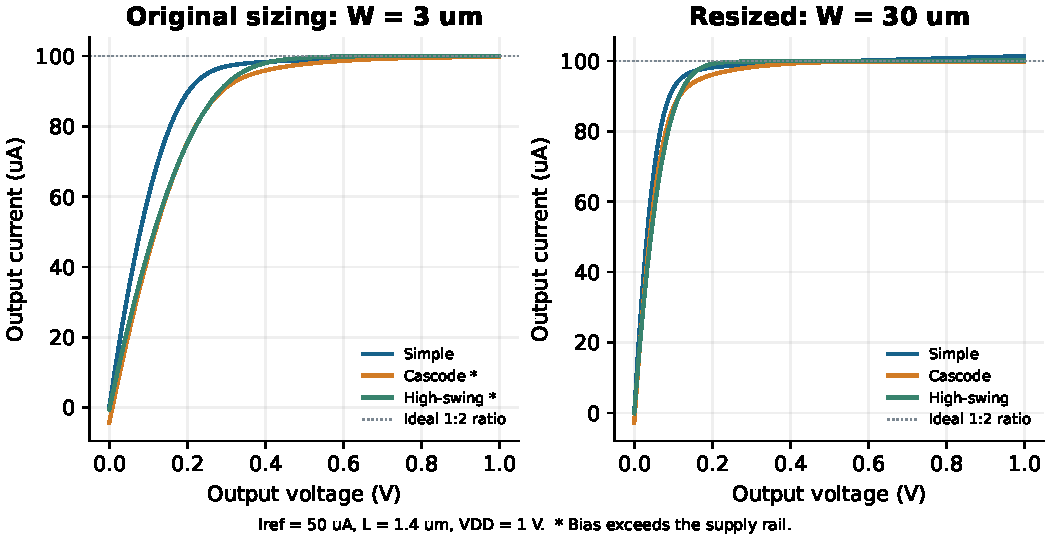
\includegraphics[width=\linewidth]{figures/aic01_mirrors.pdf}
\caption{Simple/cascode/high-swing curves redrawn from actual HSPICE DC data. Original and widened geometries both use 50 $\mu$A. Asterisks mark original cases with above-rail bias; those curves are not evidence of a passing physical 1 V implementation. This is not a WaveView screenshot.}
\end{figure}

\begin{figure}[htbp]\centering
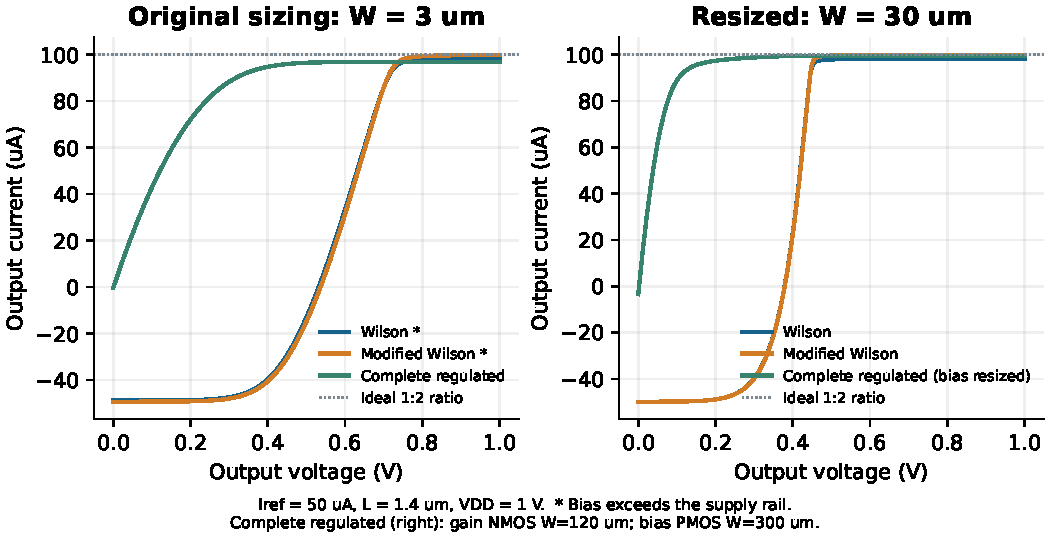
\includegraphics[width=\linewidth]{figures/aic01_feedback.pdf}
\caption{Wilson, modified Wilson and complete-regulated curves redrawn from actual DC data. Resized Wilson/modified circuits use case 3; the final complete-regulated bias sizing uses case 4. Above-rail original cases are retained only for failure analysis. This is not a WaveView screenshot.}
\end{figure}

Operational range and power for case 3, with complete-regulated case 4 added:

\begin{center}\small
\begin{tabular}{lrrrrr}
\toprule
Topology & Case & $V_{min,5\%}$ (V) & $P_b$ ($\mu$W) & $P_o$ ($\mu$W) & Rail margin (V) \\
\midrule
Simple & 3 & 0.120 & 50.000 & 80.616 & 0.560 \\
Cascode & 3 & 0.173 & 50.000 & 79.825 & 0.025 \\
High-swing & 3 & 0.141 & 100.000 & 80.050 & 0.429 \\
Wilson & 3 & 0.496 & 50.000 & 78.514 & 0.027 \\
Modified Wilson & 3 & 0.500 & 50.000 & 79.867 & 0.024 \\
Regulated & 3 & 0.498 & 100.000 & 79.923 & 0.025 \\
Complete regulated & 3 & 0.142 & 130.021 & 79.823 & 0.062 \\
Complete regulated & 4 & 0.142 & 148.327 & 79.670 & 0.120 \\
\bottomrule
\end{tabular}
\end{center}

$P_b$ and $P_o$ are separate power terms; $P_b$ must not be called total power. Cascode case 3 leaves only about 25 mV below the upper rail and does not establish compliance for a real IREF device. A blank means no interval meets the stated definition, not zero volts.

\subsection{Measurements for the Additional Questions}
The swapped-diode version at widened-geometry 50 $\mu$A and 0.8 V produces $I_o=18.1816\,\mu$A and a reference node of about 2.809 V. It therefore fails to function as a 1 V, 1:2 mirror at this operating point. This is not a proof of impossibility under every possible bias condition.

Deck 07's finite-bandwidth ideal feedback-amplifier experiment gives:

\begin{center}\small
\begin{tabular}{lrrr}
\toprule
A & $I_o$ ($\mu$A) & $R_o$ (M$\Omega$) & $V_g$ (V) \\
\midrule
1 & 57.975 & 2.415 & 0.705 \\
10 & 74.287 & 9.798 & 0.787 \\
100 & 78.141 & 51.695 & 0.809 \\
\bottomrule
\end{tabular}
\end{center}

More gain raises output impedance, but the branch with fixed $V_{set}=0.15$ V does not replicate 100 $\mu$A. Large output resistance does not imply correct current ratio. The ideal controlled source does not include real amplifier power, output swing or transistor-level stability design.

\section{Discussion}
\begin{enumerate}
\item \textbf{Identical units and layout (p7).} Equal $W,L$ reduce geometry-dependent systematic differences; parallel unit count then sets the ratio. The 1+2+4+8+16 arrangement totals 31 units. A central reference unit and symmetric pairs can place the groups at a common centroid. Use the same orientation, perimeter dummies, symmetric low-resistance routing, matched contacts and a similar thermal environment. This is layout guidance, not a GDS or mismatch verification result.
\item \textbf{High-swing M4 sizing and current error (p12).} Ignoring body effect, target $V_{bias}\simeq V_T+2V_{OV}$. At equal current, the strong-inversion square law gives $(W/L)_4\simeq(W/L)_{unit}/4$. The handout starts with a 7 $\mu$m length. Actual behavior also depends on body effect, unequal $V_{DS}$, short-channel effects and leakage; deck 04 supplies the length variants. The 1 $\mu$A cases may be Subth, where the square law should not be imposed. For question 2.4-Q2, the smaller high-swing current in the handout should be examined through its different internal $V_{DS}$ and bias conditions, finite output conductance and channel-length modulation: at equal $V_{GS}$, a smaller $V_{DS}$ can reduce the CLM current increase. This is not an inequality guaranteed by topology, and the old plot does not require this model to show the same ordering. At the common 0.8 V point, case 3 with the supplied model instead gives 100.063 $\mu$A for high-swing and 99.781 $\mu$A for conventional cascode. The opposite measured ordering is retained rather than forced to match the old conclusion.
\item \textbf{Wilson diode swapping and modification (p17).} Diode placement determines bias nodes and the feedback path; swapping the symbols does not preserve function automatically. Section 5 retains a failing example. Modified Wilson adds a matching diode to improve the lower devices' $V_{DS}$ correspondence, while the dominant output-resistance order remains $g_mr_o^2$. Case-3 Wilson/modified resistance is about 10.353/10.025 M$\Omega$, while current error improves from $-1.857\%$ to $-0.166\%$: better DC matching with a similar resistance order.
\item \textbf{Regulated comparison and power (p20, p21 Q1).} Extra feedback gain can raise $R_o$ but costs bias current, area, parasitic poles and headroom. A complete implementation can still fail when an amplifier-load transistor loses saturation, so output-current accuracy alone is insufficient. Page 20 also notes that unequal M0/M1 $V_{DS}$ still causes copying error; adding M4--M6 does not automatically remove it. Final case 4 still has $-0.413\%$ error rather than zero.
\item \textbf{Higher-order resistance (p21 Q2).} Both $g_m$ and $g_d$ have units S, making $g_m^3/g_d^5$ have units $\Omega^2$, not resistance. If the intent were one extra dimensionless gain stage, $g_m^3/g_d^4$ might be intended; this is an interpretation, not a verified correction to the handout. Deck 07 only tests the dimensionally valid concept $R_o\sim A g_mr_o^2$. A physical higher-order feedback mirror still requires clarification of the question, a transistor amplifier, loop-gain/phase checks, startup, noise, power and PVT work. The literal specification remains unresolved.
\end{enumerate}

\section{Conclusion}
The chapter-wide circuit/question mapping, seven executable decks and actual HSPICE simulations of 30 cases are complete, including the out-of-range and inaccurate results. Original geometry does not reproduce all handout results at 1 V. Explicit resizing for the supplied model improves the comparison operating points, and the complete-regulated circuit requires additional bias sizing. Only the declared measurements and operating-point checks are satisfied where stated; physical IREF design, full PVT, layout and the dimensionally inconsistent question are not claimed complete.

Traceable data are under \texttt{AIC/Lab01/results/}: per-case CSV files, exported measurement values, \texttt{comparison.csv}, \texttt{operating\_points.csv} and \texttt{simulation\_data.json}. \texttt{manifest.json} records the specification mapping and case definitions. Waveforms reveal behavior over a range; \texttt{.measure} extracts defined numerical metrics. Both are used together.
